% ICML 2026 workshop submission using the official ICML style (most ICML workshops
% accept this template; replace the workshop line with the exact workshop name from the CFP if required).
\documentclass{article}

\usepackage{graphicx}
\usepackage{booktabs}
\usepackage{hyperref}

\PassOptionsToPackage{numbers,sort&compress}{natbib}
\usepackage{icml2026}

\usepackage{amsmath}
\usepackage{amssymb}
\usepackage{placeins}

\graphicspath{{figures/}}

\icmltitlerunning{Noisy Judges in Self-Improving Idea Generators}

\begin{document}

\twocolumn[
\icmltitle{\texorpdfstring{Noisy Judges, Consistent System-Level Preference \\ in Self-Improving Scientific Idea Generators: A Trajectory Study \\[0.2em] {\large \itshape ICML 2026 Workshop (submission draft)}}{Noisy Judges, Consistent System-Level Preference in Self-Improving Scientific Idea Generators: A Trajectory Study}}

\begin{icmlauthorlist}
\icmlauthor{Anonymous}{aff}
\end{icmlauthorlist}

\icmlaffiliation{aff}{Anonymous Institution, Anonymous City, Anonymous Country}
\icmlcorrespondingauthor{Anonymous}{anon@domain.com}

\icmlkeywords{%
self-improving agents, LLM judges, scientific idea generation, evaluation noise, pairwise preference, human evaluation.
}

\vskip 0.3in
]

\printAffiliationsAndNotice{}

\begin{abstract}

Recent progress in AI development increasingly relies on iterative improvement cycles, where systems are manually modified, benchmarked, and refined through repeated experimentation. Automating this process using coding agents could dramatically accelerate development. While prior work has demonstrated self-editing systems under objective evaluation metrics, applying similar loops in subjective domains remains challenging because reliable improvement is difficult when evaluation signals are noisy and inconsistent.

To study this problem, we build an automated coding loop in which a language-model-based software engineering agent proposes and implements modifications to a scientific idea-generation system, starting from \texttt{S\_sota}, an implementation of the EvoScientist pipeline, a strong recent state-of-the-art system for scientific idea generation. Each candidate system is evaluated against the current champion using pairwise judging, and candidates that win often enough are promoted, enabling iterative improvement based solely on preference feedback. Using this process, we automatically evolve the starting system into a new version (\texttt{S15}) that is consistently preferred over the original system.

Across both automated judges and expert human raters, individual pairwise decisions show substantial disagreement at the item level. Despite this noise, the evolved system is consistently preferred over the starting system by three independent automated judges on a frozen evaluation slice and in a blind human pilot (40 of 60 comparisons). This demonstrates that improvements discovered using one evaluator can remain valid under independently constructed evaluators.

Together, these results show that automated coding loops can reliably improve strong baseline systems even when individual evaluations are noisy. More broadly, they demonstrate that stable system-level improvement signals can emerge through aggregation across many comparisons, enabling automated iterative system design in domains where objective evaluation metrics are unavailable.

\end{abstract}

\section{Introduction}

Large language models are increasingly used to automate parts of scientific discovery, including hypothesis generation, experimental planning, and manuscript drafting. Recent systems such as VirSci, The AI Scientist, Gemini Co-Scientist, and EvoScientist suggest that multi-agent research pipelines can generate plausible scientific ideas and iteratively refine them~\cite{su2024twoheads,lu2024aiscientist,gottweis2025coscientist,lyu2026evoscientist}. The open question is whether these systems can improve subjective idea quality in a way that survives evaluation stronger than the same judge signal that guided optimization.

This question matters because scientific idea generation remains difficult even when model outputs are fluent and well structured. Prior work finds that language models can propose novel-looking ideas, but reliably producing expert-level contributions is still unresolved~\cite{si2024novelideas}. In practice, improving agentic research systems still depends heavily on manual prompt and workflow tuning.

Self-improving systems offer an alternative. Rather than hand-editing a workflow indefinitely, one can evolve the workflow itself and retain only variants that outperform the current champion. The Darwin G\"{o}del Machine provides a concrete template for this style of optimization over code and agent structure~\cite{zhang2025darwin}.

We therefore study a narrower question: what survives stronger evaluation once judge noise is made explicit? At the system level, every evaluator we ran---three automated judges on a frozen slice and eight human raters on a disjoint topic pilot---prefers the evolved generator over the reboot baseline. At the item level, those evaluators disagree substantially on which specific ideas win a given topic. We argue that aggregate system-level preference can still be extracted when the protocol averages across enough pairs and independent evaluators.

\paragraph{Contributions.}
\begin{itemize}

\item We build an automated research system that improves agents using subjective evaluation signals. Using scientific hypothesis generation as our test case, we start from EvoScientist, a system reported to achieve state-of-the-art performance, and iteratively improve it to produce a version that is consistently preferred over the original under our evaluation protocol.

\item We show that the improved system is consistently preferred over the prior system across three independent automated judges and an eight-rater blind human pilot, even though those same evaluators frequently disagree on individual comparisons.

\item We analyze the structure of evaluator disagreement and show that stable system-level preference emerges through aggregation across many comparisons, despite noisy per-item labels.

\end{itemize}

\section{System and benchmark}

\subsection{Generator and benchmark slice}
\label{sec:setup}

Each system version is a Python module that combines LLM API calls with supporting logic such as literature search, critique steps, and structured idea generation. A typical generator identifies gaps in existing work, drafts candidate ideas, and refines them across multiple reasoning steps. The generator model is held fixed at \texttt{gpt-4.1-mini} for every version and every comparison, so all measured differences come from changes to the surrounding code rather than from swapping model weights.

The benchmark is a fixed set of 15 topics (\texttt{ideas/benchmark\_topics.json}). For every comparison, both the current reference system (the \textbf{champion}) and the modified system (the \textbf{candidate}) generate $n_{\text{ideas}}{=}5$ ideas per topic, yielding $N{=}75$ matched pair keys per full evaluation. Idea generation runs in parallel via a worker pool; matched outputs are stored to disk so re-judging never re-runs generation.

\subsection{Self-improvement loop (Figure~\ref{fig:harness})}

The coding agent (\texttt{swe\_agent.py}) proposes targeted edits to the champion's source: prompt revisions, retrieval changes, new reasoning steps, or larger restructurings of the generation pipeline. Each proposed edit is first screened by a \emph{mini-eval} (3 topics $\times$ 3 ideas = 9 pairs against the current champion) to discard obviously broken or regressive edits. Edits that survive several rounds of mini-eval are bundled into a candidate version $S_{n+1}$ and submitted to the \emph{full eval}.

The full eval re-uses the matched 75-pair design from \S\ref{sec:setup} and computes the tie-adjusted candidate win rate
\[
\widehat{\mathrm{WR}}_B = \frac{W_B + \tfrac{1}{2} T}{N},
\]
where $W_B$ is the number of pairs the candidate wins, $T$ is the number of ties, and $N{=}75$. Promotion is a hard threshold:
\[
\widehat{\mathrm{WR}}_B > 0.55 \;\Rightarrow\; \text{candidate becomes new champion},
\]
otherwise the candidate is rejected and its code discarded. Across the trajectory studied here, repeated applications of this loop produce versions ending at \texttt{S15}. The reboot baseline used for the second trajectory is \texttt{S\_sota} (generator module \texttt{S\_sota.py}); the from-scratch trajectory in Figure~\ref{fig:prearchive_loop} uses an earlier direct-prompt baseline \texttt{S0}.

\begin{figure*}[t]
  \centering
  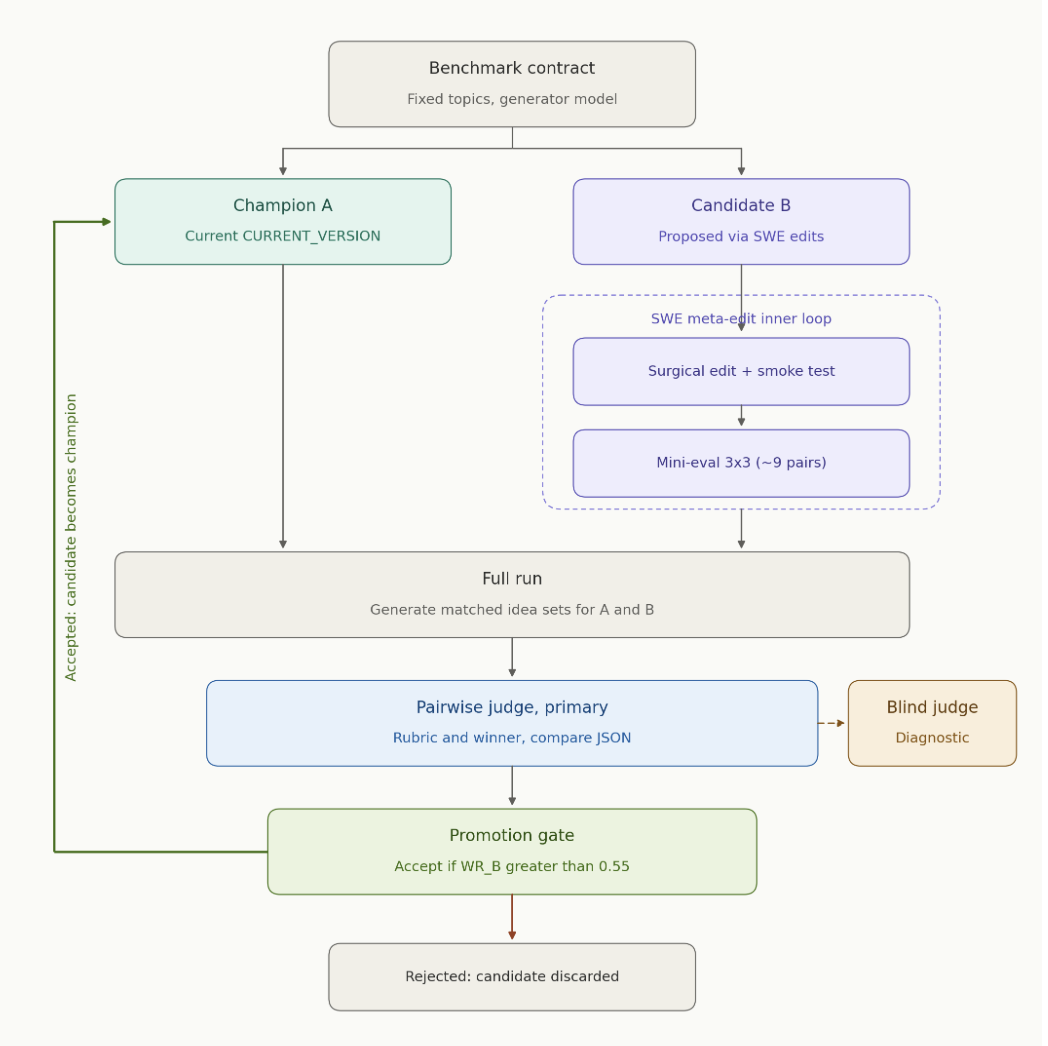
\includegraphics[width=0.88\textwidth]{system_diagram.png}
  \caption{G\"{o}del/Darwin harness: benchmark, SWE edit loop, full eval, judge, promotion gate (system diagram).}
  \label{fig:harness}
\end{figure*}

\subsection{Pairwise judging protocol}
\label{sec:judges}

Every comparison---automated or human---uses the same pairwise schema. The judge is shown a topic, Idea~A, and Idea~B, and is asked for integer scores in $[0, 10]$ on four criteria: \emph{novelty}, \emph{scientific usefulness}, \emph{experimental clarity}, and \emph{feasibility}. The winner is the side with the higher total; if totals differ by 2 or fewer points the judge must declare a tie. To control positional bias, each pair independently flips Idea~A/Idea~B presentation order with probability $\tfrac{1}{2}$ before the prompt is rendered, and the verdict is unflipped after parsing.

The \textbf{training judge} (\texttt{deepseek-chat}, temperature 0.2) is the only signal used by the promotion gate; it is the judge the loop is allowed to optimize against. The \textbf{in-loop blind judge} (\texttt{gemini-flash-lite-latest}, temperature 0.2) runs on a 5-topic sample of every full eval and is recorded alongside the training-judge verdict, but is never fed back into the promotion decision or the coding agent's prompt context. This is the open-marker series in Figure~\ref{fig:trajectory}.

\subsection{Judge feedback to the coding agent}
\label{sec:feedback}

The coding agent never sees per-pair scores. After each full eval, \texttt{swe\_agent.py} parses the stored compare report and extracts only two streams of qualitative feedback:

\begin{itemize}
  \item \emph{Judge reasoning snippets}, separated by which side won. The 2--3 sentence \texttt{reasoning} field that the judge emits with each verdict is bucketed into ``why the champion won this pair'' and ``why the candidate won this pair'' rolling lists. The most recent 20 of each are kept in \texttt{results/swe\_context.json}.
  \item \emph{An iteration log} of the last 8 candidate versions: the candidate's $\widehat{\mathrm{WR}}_B$, its accept/reject status, a one-line summary of what changed in the code, and a short excerpt of the reasoning quoted when that candidate's wins were credited.
\end{itemize}

Both streams are injected into the diagnose prompt for the next iteration so the agent's edits are conditioned on what the judge has consistently rewarded and on what previous attempts changed without paying off. Crucially, raw $\widehat{\mathrm{WR}}_B$ values from the in-loop blind judge are recorded for diagnostics but are not inserted into this prompt context, preserving it as a blind evaluation signal.

\subsection{Double-blind human evaluation}
\label{sec:human-ui}

The human pilot uses a local web UI (\texttt{human\_judge\_ui.py}) that keeps raters blind to system identity. After picking two runs and (optionally) a custom topic, the rater enters \emph{blind mode}: version names are hidden in the UI, the two picks are randomly mapped to ``left''/``right'', and each pair independently flips Idea~A/Idea~B before display. The next-pair endpoint never returns version IDs; the page merges them in only when a vote is recorded. A rater name is required on every vote so per-rater statistics can be computed offline, but it is never echoed back during scoring. The pilot used 12 expert-chosen topics scored by 8 raters on disjoint slices, totalling 60 pairwise judgments (Table~\ref{tab:margins}); the disjoint-slice design precludes inter-rater reliability on shared items, as noted in \S\ref{sec:limits}.

\FloatBarrier

\section{Results}

\subsection{Headline: system-level preference is consistent across evaluators even where item-level agreement is weak}
\label{sec:headline}

\begin{table}[t]
  \centering
  \scriptsize
  \setlength{\tabcolsep}{2pt}
  \begin{tabular}{@{}lccc@{}}
    \toprule
    Source & \shortstack[l]{\texttt{S15} (A) / \texttt{S\_sota} (B) / tie\\(three counts per row)} & $\widehat{\mathrm{WR}}_B$ (side B) & 95\% CI \\
    \midrule
    Gemini 3 Flash & 32 / 4 / 28 & 28.1\% & 16.4--40.6\% \\
    GPT-5.4        & 39 / 5 / 20 & 23.4\% & 15.7--32.3\% \\
    DeepSeek Chat  & 43 / 20 / 1 & 32.0\% & 19.9--46.4\% \\
    Human (8 raters) & 40 / 15 / 5 & 29.2\% & 18.3--40.0\% \\
    \bottomrule
  \end{tabular}
  \caption{Batch margins: evolved champion \texttt{S15} is always \textbf{side~A}; reboot baseline \texttt{S\_sota} is \textbf{side~B} (so $\widehat{\mathrm{WR}}_B$ is the tie-adjusted win rate for the baseline). Automated rows: publish-eval intersection ($N{=}64$). Human: blind pilot ($n{=}60$, disjoint topic slices).}
  \label{tab:margins}
\end{table}

Before the trajectory plot, we state the main empirical finding: on \texttt{S15} vs.\ \texttt{S\_sota}, every evaluator we ran prefers \texttt{S15} at the system level. Table~\ref{tab:margins} summarizes batch margins on a frozen publish-eval intersection ($N{=}64$ pairwise keys) for three automated judges and the human pilot ($n{=}60$). Item-level agreement between judges is weak (typical Cohen $\kappa$ on pairwise labels in the 0.07--0.21 range on that overlap), but the batch direction is stable---the pattern we expect when aggregating noisy per-pair labels.

\subsection{Two-phase improvement trajectory (Figure~\ref{fig:prearchive_loop}, Figure~\ref{fig:trajectory})}

We analyze the behavior of the automated coding loop across two development phases: an initial run starting from a baseline system (Figure~\ref{fig:prearchive_loop}) and a second run starting from a stronger state-of-the-art system (Figure~\ref{fig:trajectory}). Each point in the trajectory corresponds to a candidate system version proposed by the coding agent and evaluated against the current champion.

\paragraph{Phase I: baseline improvement (Figure~\ref{fig:prearchive_loop}).}
The first trajectory begins from a baseline generator and tests whether iterative code modifications can produce measurable improvements. Early iterations produce large gains, followed by a mixture of accepted and rejected candidates as performance stabilizes. The presence of rejected candidates indicates that the promotion gate filters unhelpful edits rather than accepting changes indiscriminately. Over time, improvements become smaller and less frequent, suggesting convergence toward a locally refined configuration.

\begin{figure*}[t]
  \centering
  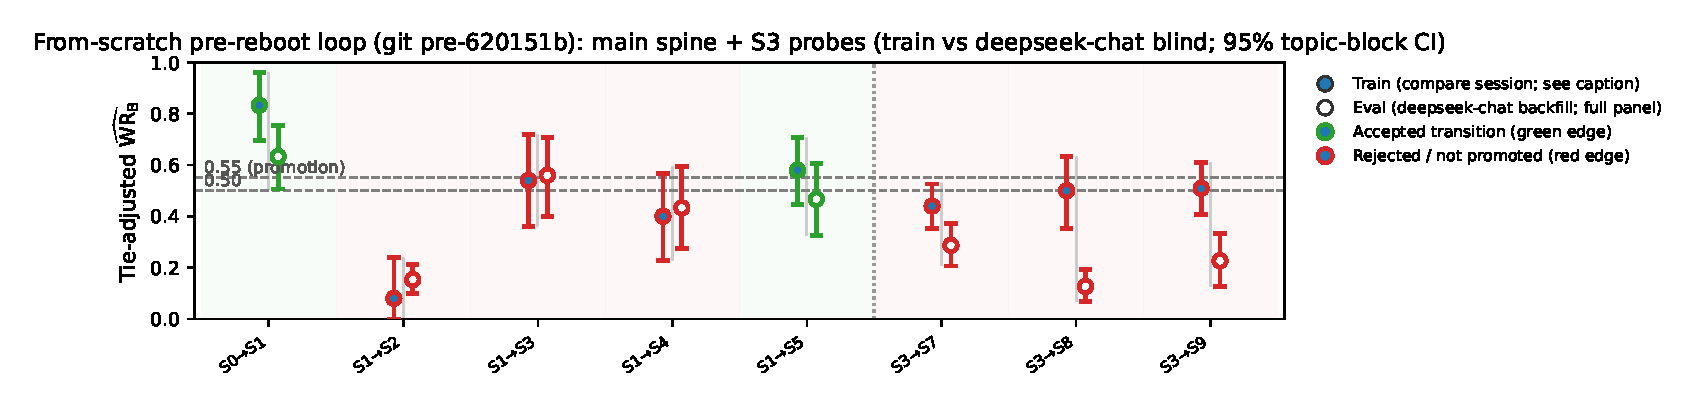
\includegraphics[width=0.95\textwidth]{figure1_prearchive_loop_trajectory_wr.pdf}
  \caption{\textbf{Separate lineage, not \texttt{S\_sota}:} an \emph{independent} Gödel-loop run implemented from scratch with direct-prompt baseline \texttt{S0} and archived before the clean-slate reboot (git parent of \texttt{620151b}). It is \textbf{not} the continuation of Figure~\ref{fig:trajectory}, which starts from the reboot champion \texttt{S\_sota} (first promotion \texttt{S\_sota}$\to$\texttt{S12}). Left of dotted line: main promotion spine through \texttt{S5} (\textbf{no} \texttt{S6}). Right: same-era archived \texttt{S3} vs.\ \texttt{S7}/\texttt{S8}/\texttt{S9} probe compares (\texttt{S3} was a rejected candidate; not a linear \texttt{S5}$\to$\texttt{S7} chain). Filled: historical compare sessions; open: \texttt{deepseek-chat} blind backfill.}
  \label{fig:prearchive_loop}
\end{figure*}

Figure~\ref{fig:prearchive_loop} serves as descriptive background, illustrating how a from-scratch evolution behaved under an earlier code snapshot. The main results reported in Table~\ref{tab:margins} and Figure~\ref{fig:trajectory} correspond to the post-reboot trajectory seeded from \texttt{S\_sota} under the current harness; the two trajectories should not be interpreted as a single continuous run.

\paragraph{Phase II: refinement from state-of-the-art (Figure~\ref{fig:trajectory}).}
After refining the coding agent during Phase I, we restart the loop from a stronger reference system (\texttt{S\_sota}). This phase tests whether meaningful improvements can still be discovered when starting from an already strong system.

In this regime, most candidate edits are rejected and successful promotions occur less frequently than in the baseline phase, as expected near high-performing systems. Nevertheless, several successful promotions occur, demonstrating that improvements remain possible even when starting from a strong baseline.

\begin{figure*}[t]
  \centering
  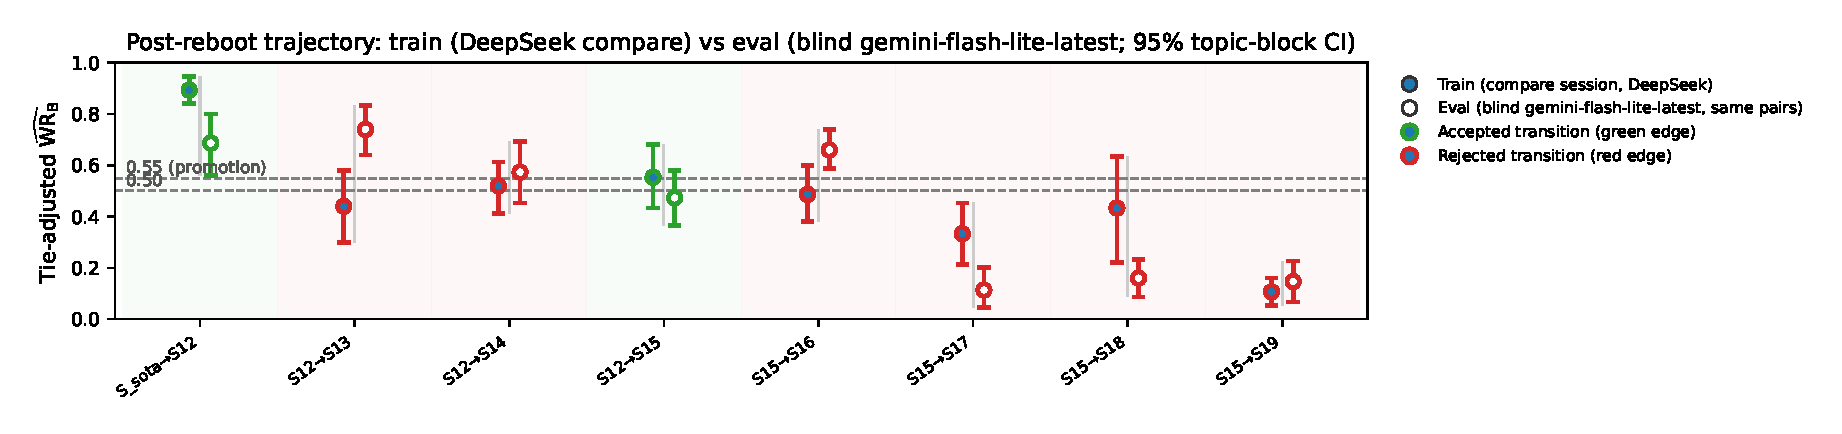
\includegraphics[width=0.92\textwidth]{figure1_trajectory_wr.pdf}
  \caption{Post-reboot trajectory (seeded from \texttt{S\_sota}, not the from-scratch \texttt{S0} line in Figure~\ref{fig:prearchive_loop}): tie-adjusted candidate win rate $\widehat{\mathrm{WR}}_B$ per promotion decision (training judge vs.\ blind re-evaluation).}
  \label{fig:trajectory}
\end{figure*}

Each point represents one candidate system that was tested against the current champion. Filled markers show the scores from the training judge, which determines whether a candidate is promoted. Open markers show scores from an independent blind judge that was not used during optimization.

Only two candidates were promoted in this trajectory: the transition from \texttt{S\_sota} to \texttt{S12}, and later from \texttt{S12} to \texttt{S15}. Most other candidates were rejected. This differs from the earlier from-scratch trajectory, where improvements were larger and promotions happened more frequently. Starting from a strong baseline makes further improvements harder to find, so fewer candidates succeed.

Most of the overall improvement occurs at the first accepted step, from \texttt{S\_sota} to \texttt{S12}. This transition produces the largest separation from the baseline. The later step from \texttt{S12} to \texttt{S15} is weaker. It is borderline according to the training judge and close to neutral according to the blind judge. This suggests that early modifications account for most of the gain, while later changes provide smaller refinements.

Importantly, the accepted steps remain directionally consistent when evaluated by the blind judge. Although the blind scores are often closer to neutral than the training scores, they do not reverse the promotion decisions. This suggests that the observed improvements are not limited to the specific judge used during training.

\subsection{Disagreement structure and system-level consistency}
\label{sec:agree}
\label{sec:judge_human}

We next examine the structure of disagreement across evaluators to understand how noisy pair-level judgments contribute to the system-level consistency observed earlier.

\begin{figure*}[t]
  \centering
  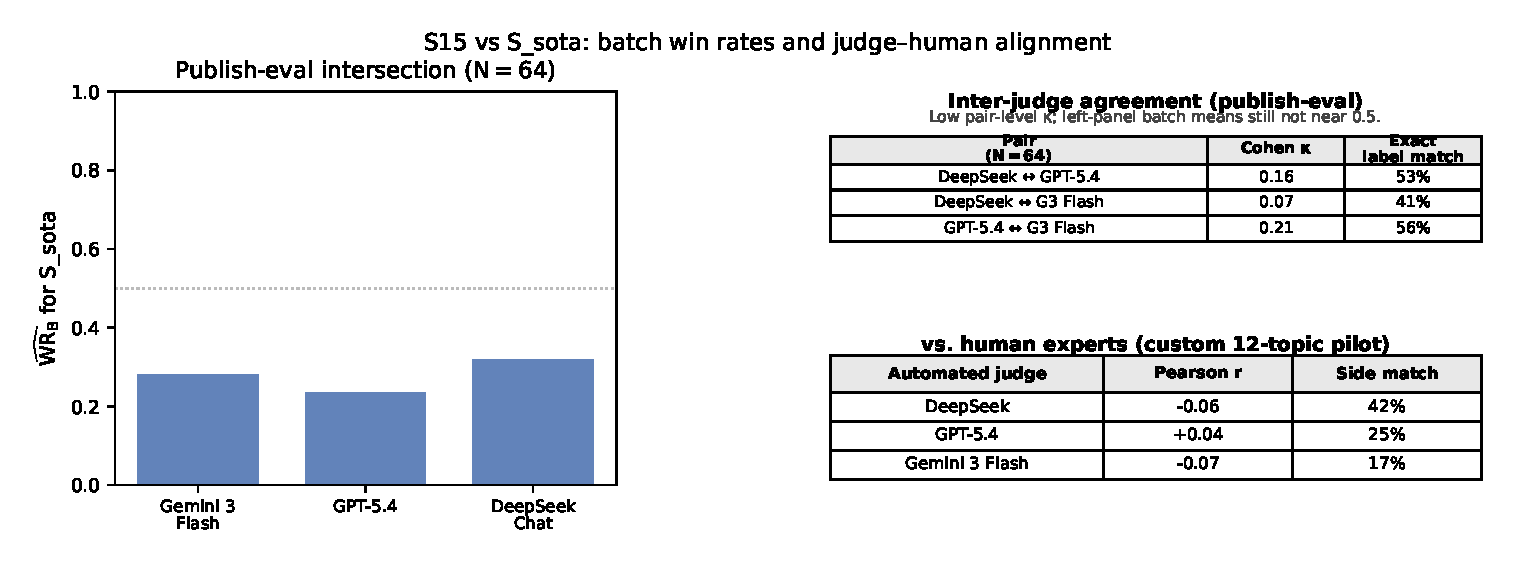
\includegraphics[width=0.95\textwidth]{figure2_human_vs_llm.pdf}
  \caption{\textbf{Left:} batch $\widehat{\mathrm{WR}}_B$ for \texttt{S\_sota} on the $N{=}64$ frozen publish-eval slice (same judges as Table~\ref{tab:margins}). \textbf{Top right:} pair-label Cohen $\kappa$ between judges on that overlap. \textbf{Bottom right:} per-topic win-rate correlation and side-match vs.\ the human pilot (12 topics, disjoint raters).}
  \label{fig:batch_kappa}
\end{figure*}

Figure~\ref{fig:batch_kappa} shows that agreement between automated judges is low at the level of individual comparisons. On the shared set of 64 publish-eval pairs, Cohen's $\kappa$ between judge pairs falls in the range 0.07 to 0.21, indicating that different judges frequently select different winners for the same pair. This level of agreement is consistent with visibly noisy item-level labels rather than stable per-pair verdicts.

We also compare automated results to human evaluations collected on a separate pilot. The human study includes 60 pairwise comparisons across 12 expert-selected topics, scored by eight raters working on disjoint topic slices. Within this pilot, \texttt{S15} is selected in 40 of 60 comparisons, but because raters scored disjoint items, the design does not allow direct estimation of inter-rater agreement on shared pairs.

At the topic level, automated win rates show little correlation with human topic-level outcomes (Figure~\ref{fig:batch_kappa}, bottom right). Some topics that favor \texttt{S15} under automated judging do not do so under human scoring, and vice versa. This weak correlation indicates that evaluators differ not only in individual pair decisions but also in how they weight different topics.

Despite these disagreements, evaluators remain broadly consistent at the system level. Individual judgments vary substantially, but when aggregated across many pairs and topics, they continue to produce similar directional outcomes. This pattern helps explain how stable system-level preference can emerge even when agreement on individual items is weak.

\section{Conclusion}

Taken together, these results show that reliable system-level improvement can be achieved even when individual evaluations are noisy and inconsistent. The key requirement is not stable per-instance agreement, but evaluation protocols that aggregate many independent comparisons. This provides a practical foundation for iterative improvement in subjective domains where objective metrics are unavailable.

\section{Limitations}
\label{sec:limits}


\begin{itemize}

\item We evaluate a single generator-model family (\texttt{gpt-4.1-mini}) together with a limited set of automated judges. Although system-level preference remains consistent across three independently constructed judges and the human pilot, generalization to other generator architectures and larger judge panels remains an open question.

\item The human evaluation is a small pilot rather than a benchmark-scale study: 60 pairwise judgments across 12 expert-selected topics, scored by eight raters on disjoint slices. Because raters did not score shared items, inter-rater reliability on identical comparisons cannot be estimated, and the pilot should not be interpreted as a precise estimate of effect size.

\item The experiments focus on a single application domain, scientific idea generation. Whether similar aggregation behavior holds in other agentic settings—such as coding, theorem proving, or planning—remains to be tested.

\item While multiple development trajectories were examined, including both from-scratch and rebooted runs, we do not perform systematic replication across many independent restarts. The stability of the observed behavior across larger numbers of independent trajectories therefore remains an open question.

\item We do not explicitly test adversarial behavior against the judges, nor perform extensive ablations on the improvement agent itself. As a result, the system should not be interpreted as robust to Goodhart-style exploitation or optimization against flawed evaluators.

\end{itemize}

\section{Reproducibility}

\path{REPRODUCE.md} documents the regeneration commands for all headline numbers. The key frozen artifacts include \path{ideas/results/evolution_log.jsonl}, files matching \path{ideas/results/compare_*.json}, \path{ideas/results/human_blind_scores.jsonl}, and directories under \path{ideas/results/publish_eval_*}. Model IDs are pinned in \path{ideas/paper_config.py}. Wall-clock time depends strongly on API concurrency and judge-model latency, so we report the exact commands and artifact paths rather than a single fixed runtime estimate.


\begingroup
\small
\bibliographystyle{icml2026}
\bibliography{main}
\endgroup

\end{document}
